% !TeX spellcheck = en_US
\chapter{Fundamental definitions and conceptual problems}
\label{ch:fundamentaldefinitions}

While analyzing the two case studies, we remarked that
\begin{itemize}
	\item The \textit{alternatives are generated combining elements of alternative} and there is always an alternative zero (leaving the system as is)
	
	\item The \textit{scenarios are generated combining elements of scenario}
	
	\item The \textit{impacts are generated combining indicators} and \textit{indicators are organized into a hierarchy}
	
	\item \textit{Each configuration generates an impact} through descriptive models
	
	\item \textit{Decision-makers should never ignore stakeholders} (people affected by the decision and can react to it)
	
	\item \textit{Preferences are expressed on impacts} (not on configurations)
\end{itemize}

\section{Decision problem}
\label{sec:decproblemdef}

\begin{definition}
	A \textbf{decision problem} is defined by a 6-uple
	$$ P = \left(X, \Omega, F, f, D, \Pi \right)$$
	where: 
	\begin{itemize}
		\item $X$ is the \textbf{feasible region}, the set of all alternatives; 
		
		\item $\Omega$ is the \textbf{sample space}, the set of all possible scenarios, or outcomes
		
		\item $F$ is the \textbf{indicator space}, the set of all possible impacts
		
		\item $f: X \times \Omega \rightarrow F$ is the \textbf{impact function}
		\begin{itemize}
			\item every pair $(x, \omega) \in X \times \Omega$ describes a configuration of the system on which a decision should be taken
			
			\item $f$ associates to each configuration $(x, \omega)$ of the system an impact $f(x, \omega) \in F$
			
			\item impact $f(x, \omega)$ describes all the features of the configuration $(x, \omega)$ that are relevant for the decision (costs, profit, quality levels, \dots)
		\end{itemize}
		
		\item $D$ is the \textbf{set of all decision-makers}, or stakeholders
		
		\item $\Pi: D \rightarrow 2^{F \times F}$ is the \textbf{preference function}, a function that associates to each decision maker $d \in D$ a subset of impact pairs $\Pi(d) \subseteq F \times F$; this is interpreted as a binary relation representing the preference of decision maker $d$
	\end{itemize}
\end{definition}

The aim of the problem is to identify a solution $x^\ast \in X$ ir a subset of solutions $X^\ast \subseteq X$ that the decision-makers consider satisfactory based on their preferences between the impacts $f(x^\ast, \omega)$ with $\omega \in \Omega$ and the other impacts $f \in F$

\subsection{Alternatives}
\label{subsec:alternativesdef}

The alternatives formally describe the events under the control of the decision-makers. The set $X$ includes al the possible choices.

We'll assume that 
$$ X \subseteq \R^n \Leftrightarrow x = \left[x_1 \dots x_n \right]^T \text{ with } \ x_i \in \R \quad \forall i \in \{1, \dots, n\} $$
with a finite number $n$ of elements of alternative or decision variables. Real number can model several different situations (e.g. binary, enumerative, qualitative, quantitative, functions within families).

Several \textbf{kinds of feasible regions} $X$ exist
\begin{itemize}
	\item Continuous
	
	\item Discrete
	\begin{itemize}
		\item Infinite
		
		\item Finite
		\begin{itemize}
			\item Combinatorial (typically $|X| \in \Omega(d^n)$ for some $d > 1$)
			
			\item "Finite" (typically $|X| \in O(1)$)
		\end{itemize}
	\end{itemize}
\end{itemize}
Focusing on a specific kind allows algorithms which are more effective and less general.

The notation is, so far, purely descriptive and not used to make computations.

\subsection{Scenarios}
\label{subsec:scenariosdef}

The scenarios formally describe the events out of the control of the decision-makers that have non-indifferent effect on the system. The set $\Omega$ defines all such events during the time horizon relevant to the decision. Scenarios also describe modeling errors (disturbances).

We'll assume 
$$ \Omega \subseteq \R^r \Leftrightarrow \omega = \left[\omega_1 \dots \omega_r \right]^T \text{ with } w_k \in \R \quad \forall k \in \{1, \dots, r\} $$
with a finite number $r$ of elements of scenario or exogenous variables.

\subsection{Impacts}
\label{subsec:impactsdef}

The impacts formally describe all aspects that are relevant for the decision, i.e., decisions are taken based on the impact. 

The impacts are described quantitatively as vectors of real numbers. We'll assume 
$$ F \subseteq \R^p \Leftrightarrow f = \left[f_1 \dots f_p\right] \text{ with } f_I \in \R $$
with a finite number $p$ of 
\begin{itemize}
	\item indicators
	
	\item criteria
	
	\item attributes
	
	\item objectives
\end{itemize}

\subsection{Impact function}
\label{subsec:impactfunctiondef}

The impact function $f: X \times \Omega \rightarrow F$ is a vectorial function that associates each configuration $(x, \omega)$ to an impact $f(x, \omega)$. 

Trivial example
\begin{itemize}
	\item buy quantities $x_i$ of products ($n$ decision variables)
	
	\item Pay costs $\omega_i$ ($r = n$ exogenous variables)
	
	\item The total (mono-dimensional $p=1$) cost is $f(x, \omega) = \sum_{i=1}^n \omega_i x_i$
\end{itemize}

The impact function can be
\begin{itemize}
	\item a mathematical expression that describes a computation 
	
	\item a simulation or integration software
	
	\item an empirically generated graph or table
\end{itemize}

Two classical representations for finite problems are 
\begin{enumerate}
	\item The \textbf{evaluation matrix}
	\begin{center}
		\begin{tabular}{@{}l|rrrrrr@{}}
			\toprule
			\(f(x,\omega)\) & \(f_1\) & \(f_2\) & \(f_3\) & \(f_4\) & \(f_5\) & \(f_6\) \\
			\midrule
			\((x',\omega')\)   & 10 &  5 & 40 & 20 & 24 & 180 \\
			\((x',\omega'')\)  & 16 & 10 & 60 & 16 & 20 & 190 \\
			\((x'',\omega')\)  & 20 &  6 & 23 &  8 & 17 & 230 \\
			\((x'',\omega'')\) & 24 &  8 & 50 & 12 & 10 & 100 \\
			\bottomrule
		\end{tabular}
	\end{center}
	
	\item The \textbf{radar chart}
	\begin{center}
		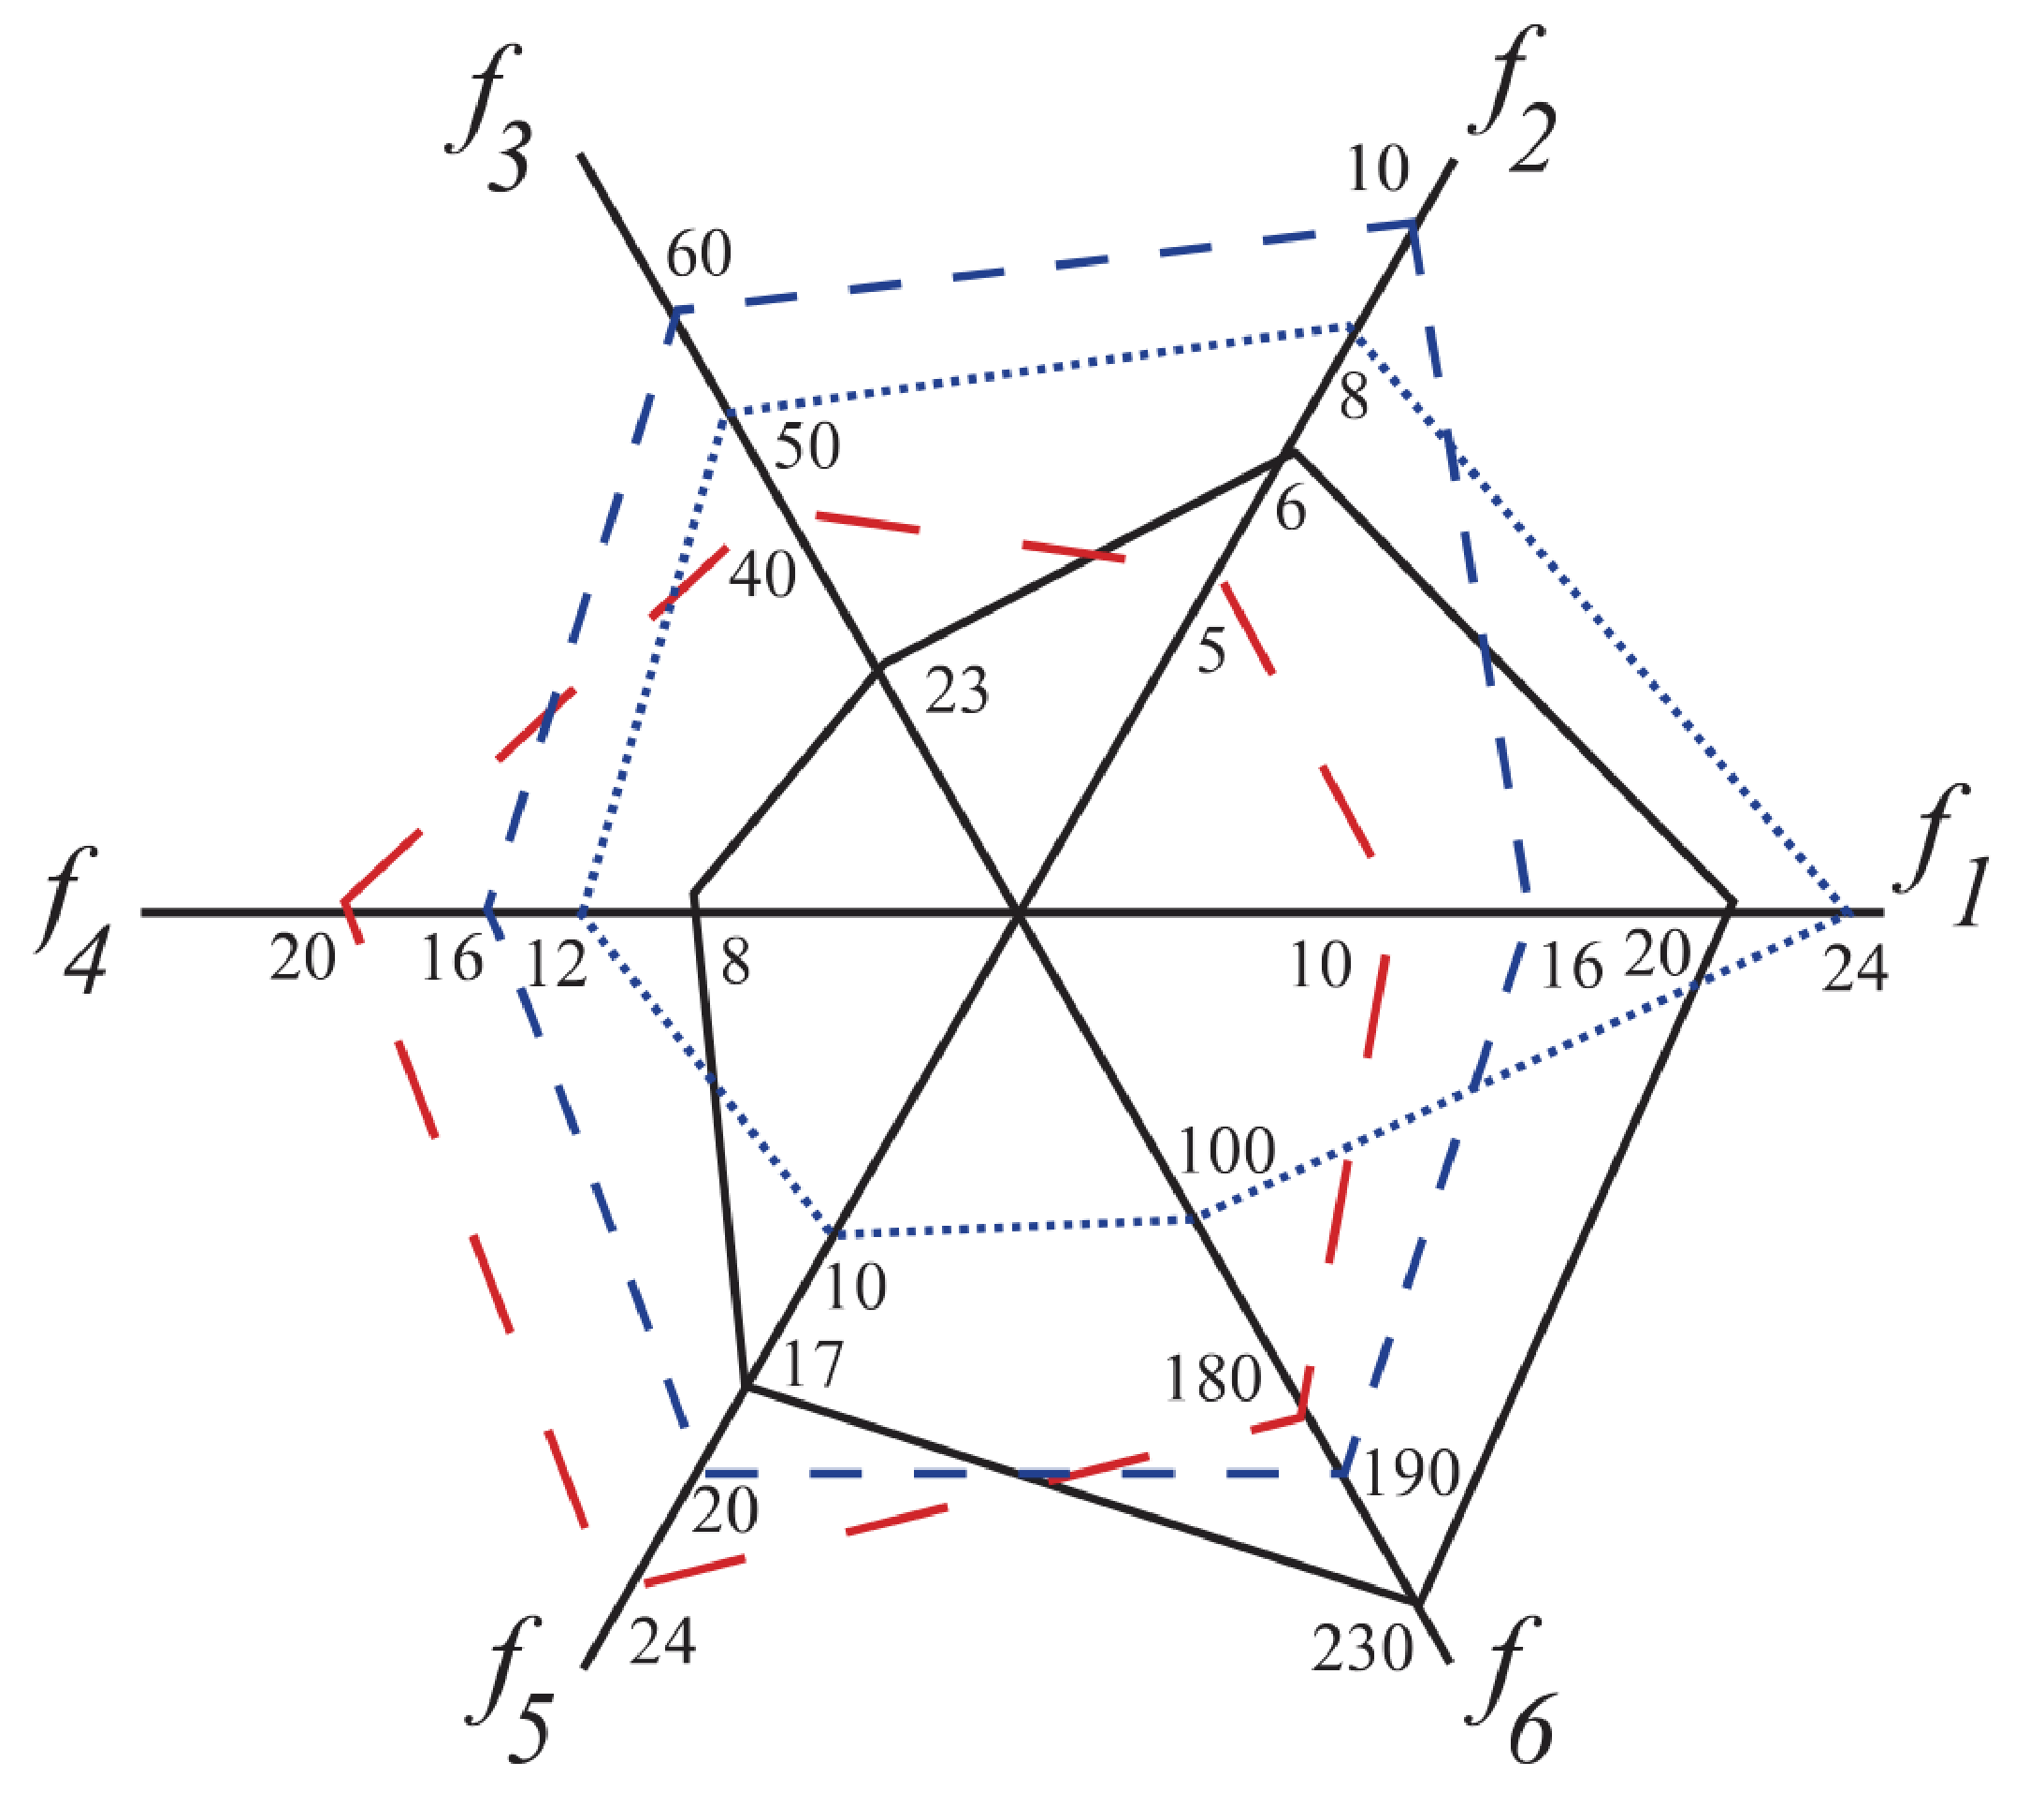
\includegraphics[width=0.45\columnwidth]{img/dp/fundamentaldefinitions/chart1}
	\end{center}
\end{enumerate}

\subsection{Decision-makers or stakeholders}
\label{subsec:decisionmakersdef}

A decision-maker is whoever takes part in a decision. The subjects who do not directly contribute to a decision, but play a role in it with their preferences are often denoted as stakeholders.

$D$ is a finite set which includes all stakeholders. They (directly or indirectly) set the value of the decision variables $x$
\begin{itemize}
	\item independently
	$$ X = X^{(1)} \times \dots \times X^{(d)} $$
	
	\item cooperatively
	$$ X = X^{(1)} \cap \dots \cap X^{(d)} $$
\end{itemize}

\subsection{Preference relation}
\label{subsec:prefreltiondef}

For each decision-maker, there is the need to distinguish \textit{which impact is preferred}, i.e., preferring $f \in F$ to $f' \in F$ means \textit{considering acceptable the replacement of $f'$ with $f$}. This corresponds to establishing a relation between pairs of impacts.

$\Pi: D \rightarrow 2^{F \times F}$ associates each decision-maker $d \in D$ to a subset of impact pairs that represents a binary relation $\Pi (d)$ on $F$.

Subset $\Pi(d) \in 2^{F \times F} \Leftrightarrow \Pi(d) \subseteq F \times F$ collects the specific pairs of impacts between which $d$ has a weak preference
$$ \Pi_d = \{(f, f') \in F \times F \mid d \text{ weakly prefers } f \text{ to } f'\} $$

\begin{definition}
	A \textbf{weak preference} is when $d$ accepts to cede $f'$ for $f$ (not strict)
	$$ f \wpref{d} f' \Leftrightarrow (f, f') \in \Pi_d$$
\end{definition} 

In the finite case, a preference relation can be represented by
\begin{enumerate}
	\item an \textbf{incidence matrix} (rows and columns are impacts, the ones are preferences)
	\begin{center}
		\begin{tabular}{@{}l|rrrrr@{}}
			\toprule
			& $f$ & $f'$ & $f''$ & $f'''$ & $f''''$ \\
			\midrule
			$f$   & 1 &  0 & 1 & 1 & 1 \\
			$f'$  & 0 & 1 & 1 & 1 & 1 \\
			$f''$  & 0 &  0 & 1 &  1 & 1 \\
			$f'''$ & 0 &  0 & 0 & 1 & 0 \\
			$f''''$ & 0 & 0 & 1 & 1 & 1 \\
			\bottomrule
		\end{tabular}
	\end{center}
	
	\item a \textbf{preference graph}
	\begin{center}
		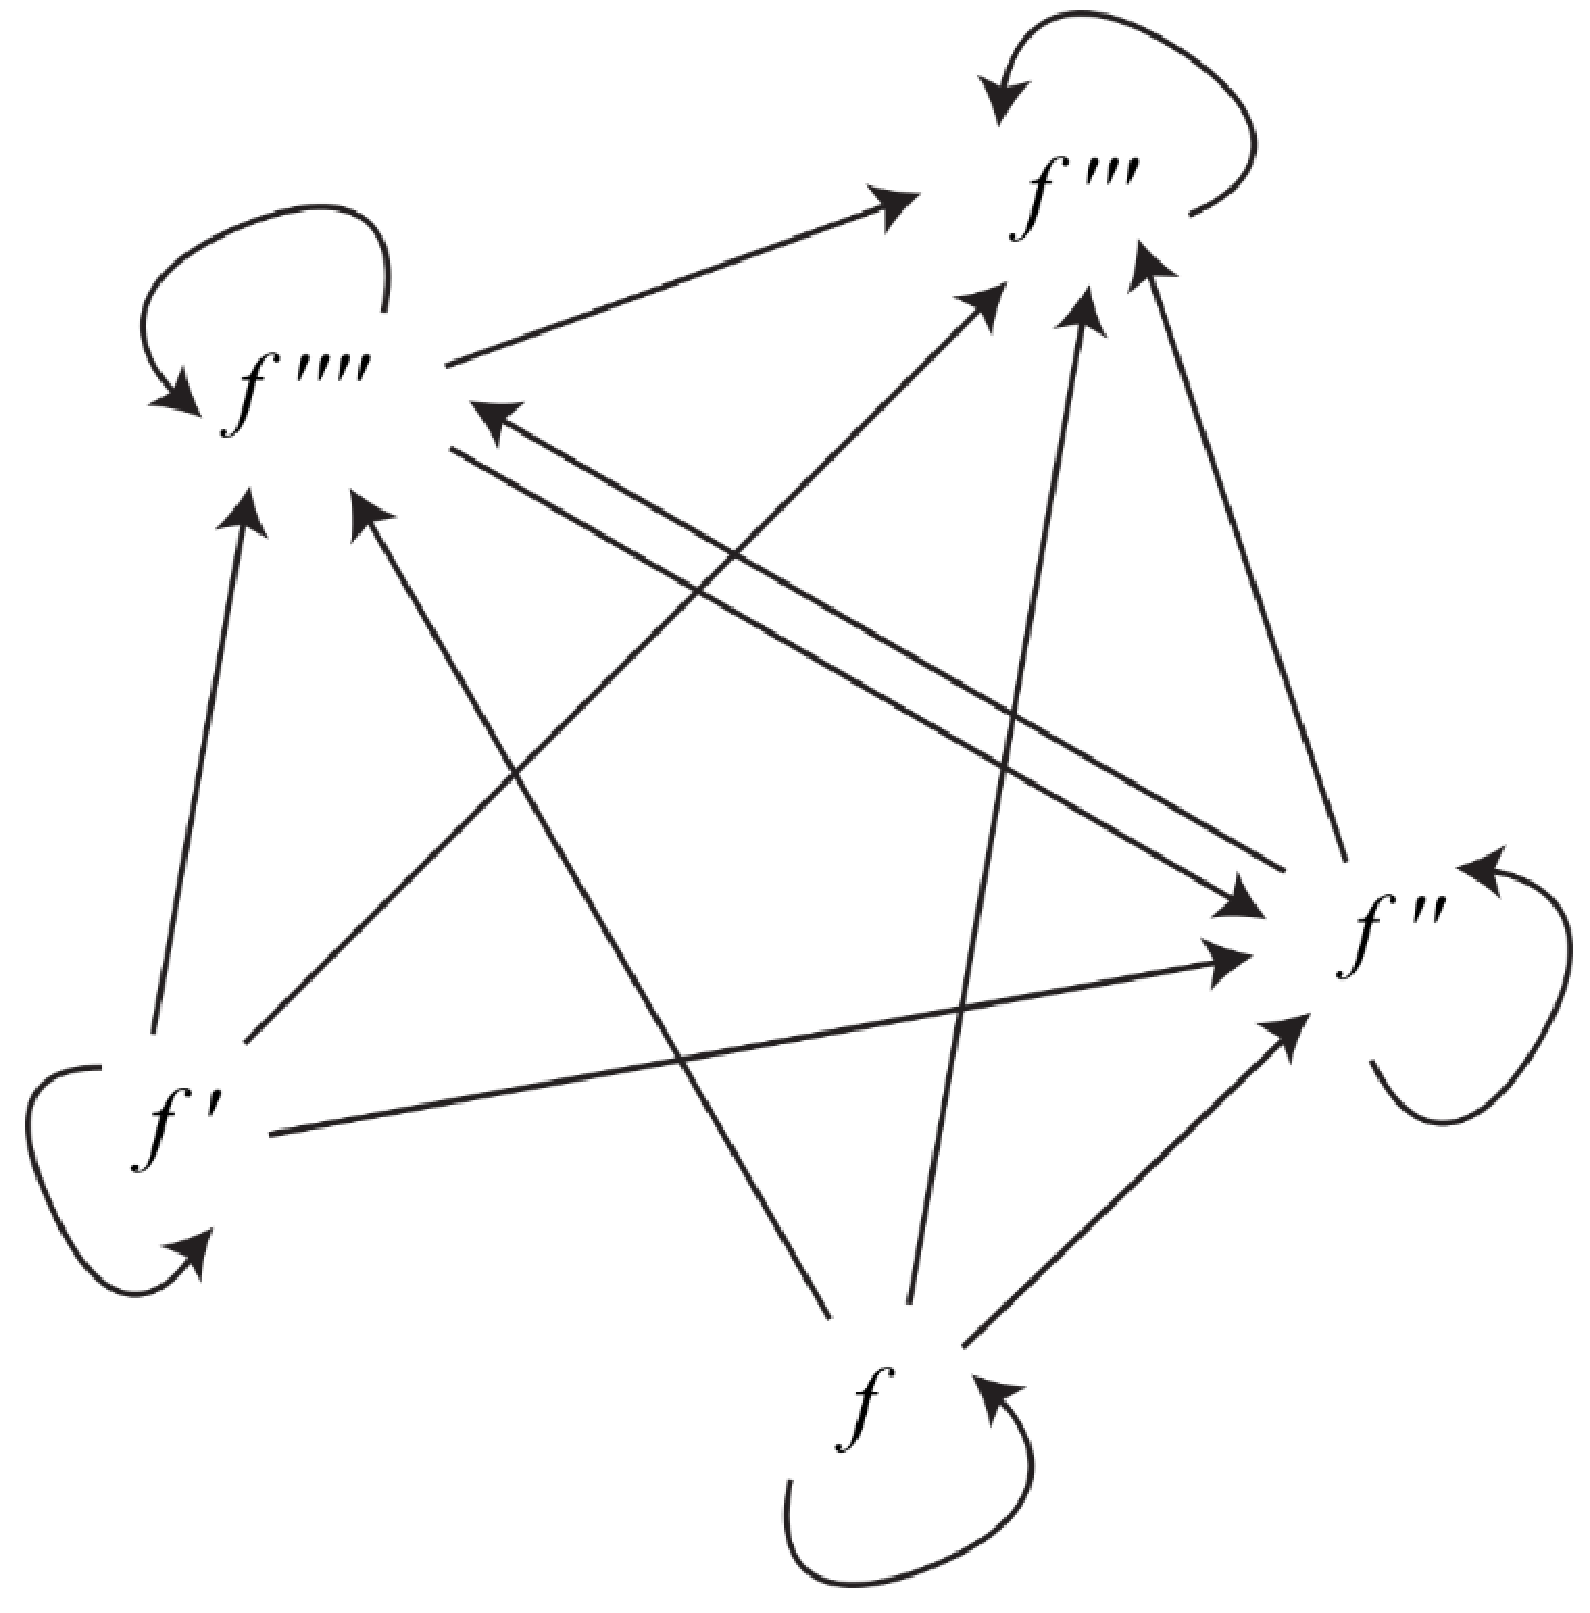
\includegraphics[width=0.45\columnwidth]{img/dp/fundamentaldefinitions/graph1}
	\end{center}
\end{enumerate}

\subsubsection{Derived relations}
\label{subsubsec:derivedrelations}

From the weak preference relation, one can derive
\begin{itemize}
	\item \textbf{Indifference} relation ($\indiff{\Pi} = \Pi \cap \Pi^{-1}$), definition:
	$$ f \sim f' \Leftrightarrow f \wpref{} f' \text{ and } f' \wpref{} f $$
	\textit{The decision-maker accepts the exchange in both directions}
	
	\item \textbf{Strict preference} relation ($\spref{\Pi} = \Pi \setminus \Pi^{-1}$), definition
	$$ f \prec f' \Leftrightarrow f \wpref{} f' \text{ and } f' \not \wpref{} f $$
	\textit{The decision-maker accepts the exchange only in the given direction}
	
	\item \textbf{Incomparability} relation ($\inc{\Pi} = \bar \Pi \cap \bar \Pi^{-1}$), definition
	$$ f \bowtie f' \Leftrightarrow f \not \wpref{} f' \text{ and } f' \not \wpref{} f $$
	\textit{The decision-maker rejects the exchange in both directions} (the decision-maker is not indifferent between the impacts, but is unable or unwilling to chose between them, refusing both exchanges)
\end{itemize}

\subsection{Property of binary relations}
\label{subsec:propertybinrel}

Not all binary relations express reasonable preference relations for a decision-maker. In principle, the preference relation should be 
\begin{itemize}
	\item \textit{Realistic}, it models correctly the aims of the decision-maker
	
	\item \textit{Effective}, it allows algorithms that yield a satisfactory choice
\end{itemize}

The two are, surprisingly, often conflicting.

Some preference relations enjoy some other special properties
\begin{itemize}
	\item \textbf{Reflexivity}: $f \wpref{} f$, $\forall f \in F$; it would be meaningless to consider a decision-maker unable to compare an impact to itself
	
	\item \textbf{Antisymmetry:} if $f \wpref{} f'$ and $f' \wpref{} f$, then $f = f'$ for all $f, f' \in F$; two impacts are indifferent only if they are identical
	
	\item \textbf{Completeness:} if $f \not \wpref{} f'$, then $f' \wpref{} f$ for all $f, f' \in F$; it requires the decision-maker to be able to always sort the impacts, though allowing ties; this excludes incomparability
	
	\item \textbf{Transitivity:} if $f \wpref{} f'$ and $f' \wpref{} f''$, then $f \wpref{} f''$, for all $f, f', f'' \in F$; discussed later
\end{itemize}

While building the model, we must investigate whether they hold or not, because they could be
\begin{itemize}
	\item useful to simplify the computation
	
	\item but unrealistic for the given problem
\end{itemize}

\paragraph{Main kinds of preference relation} Combining these properties, we can identify different kinds of preferences:
\begin{itemize}
	\item A \textbf{preorder} enjoys reflexivity and transitivity
	
	\item a \textbf{partial order} enjoys reflexivity, transitivity and antisymmetry; example: subset inclusion
	
	\item a \textbf{weak order} enjoys reflexivity, transitivity and completeness; example: rankings in sport
	
	\item a \textbf{total order} enjoys reflexivity, transitivity, antisymmetry and completeness; example: number sizes
\end{itemize}

\paragraph{Conceptual problems on transitivity} Transitivity is the most common assumption for a preference relation, and is often interpreted as an equivalent for rationality.

Rational decision-makers are transitive, humans are not. There are two main approaches to deal with this point:
\begin{enumerate}
	\item \textit{humans should be transitive}, i.e., use thought experiments to show the evil consequences of giving up transitivity
	
	\item \textit{let humans be non-transitive}, i.e., appeal to practical and thought experiments and adopt weaker models of rationality
\end{enumerate}

%End of L3
